\cleardoublepage

\section{记号}

\begin{enumerate}
      \item 我们记$x\in[0,1]$以$b$为基数的展开形式为$x=0.x_1x_2\cdots x_n\cdots$,其中$x_i\in\{0,1,\cdots,b-1\}$,也就是说$x=\underset{i=1}{\overset{\infty}{\sum}}x_ib^{-i}$。
      \item 对区间$I$,我们用$|I|$表示区间的长度。
      \item 给定区间族$\mathbb{I}=\{I_1,I_2,\cdots,I_N\}$,若$\frac{|I_i|}{|I_j|}\in\mathbb{Q}.\forall i,j$,则定义
      $$
            gcd(\mathbb{I})=\sup\{T:\frac{|I_i|}{T}\in\mathbb{Z},i=1,2,\cdots,N\}.
      $$
      \item 对区间族$\mathbb{I}$中的区间$I_i$,我们定义
      $$
            n(I_i)=\frac{|I_i|}{|\mathbb{I}|},i=1,2,\cdots,N.
      $$
      \item 我们定义区间族$\mathbb{I}$的基本区间总数量为
      $$
            n(\mathbb{I})=\sum_{i=1}^Nn(I_i).
      $$
      \item 对一个函数$f(x)$,我们定义其水平集为$L(y)=\{x:f(x)=y\}$。
      \item $\lfloor x \rfloor$表示不超过$x$的最大整数。
      \item $S(a,R)$表示以$a$为中心,边长为$2R$的正方形。
      \item $B(a,R)$表示以$a$为球心,半径为$R$的球。
      \item $\Gamma_T$表示函数$T(x)$的图像,即$\Gamma_T=\{(x,y):y=T(x)\}$。
      \item 对$F$,$N_r(F)$表示以半径为$r$的球对$F$进行覆盖所需的最小覆盖数。
      \item 对$F$,我记以下为其相邻正方形覆盖数:
      $$
            N(F\cap S(a,R),r)=\Big|\{(i,j)\in\mathbb{Z}^2\cap[0,\lfloor\frac{R}{r}\rfloor]^2:\\
                  S((a-\frac{R}{2}+\frac{r}{2}+ir,a-\frac{R}{2}+\frac{r}{2}+jr),r)\cap F\neq\emptyset\}\Big|.
      $$
      由于$\exists C>0$,使得$C^{-1}N_r(F\cap B(a,R))\le N(F\cap S(a,R),r)\le CN_r(F\cap B(a,R))$,在本文中我们用更方便的相邻正方形覆盖数替代球覆盖数。
\end{enumerate}

\section{预备知识}
\subsection{可分割折线函数}

$h(x)$周期为1,且关于$x=\frac{1}{2}$对称,在$[0,1]$区间上其为连续折线函数,且满足$h(0)=h(1)$。

同时,根据不可导点对$[0,1]$区间进行划分,可以得到$\mathbb{I}=\{I_1,I_2,\cdots,I_N\}$,$h(x)$满足$\mathbb{I}$具有基本区间长度。

满足以上性质的函数$h(x)$称为可分割折线函数。

\subsection{Littlewood多项式}
若$ab$为$k-1$阶Littlewood多项式的根,则$ab$满足:
$$
      \sum_{n=0}^{k-1}\epsilon_n(ab)^n=0.
$$
其中,$\varepsilon_n\in\{-1,1\},n=0,1,\cdots,k-1$。

\subsection{维数定义}
\subsubsection{盒维数}
对集合$F$,其的盒维数为:
$$
      \mathrm{\dim_B}F=-\frac{\log N_r(F)}{\log r}.
$$

\subsubsection{Hausdorff维数}
对集合$F$,其Hausdorff维数为:
$$
      \mathrm{\dim_H}F=\sup\{s:\forall\delta>0,\exists\{U_i\}_{i=1}^\infty,\mbox{使得}\bigcup_{i=1}^\infty U_i\supset F,\mbox{且}\sum_{i=1}^\infty (\mathrm{diam}~U_i)^s<\delta\}.
$$

\subsubsection{Assouad维数}
对集合$F$,其Assouad维数为:
$$
      \mathrm{\dim_A}F=\sup\{s:(\exists C>0)(\forall R>0)(\forall r\in(0,R))(\forall x\in F),N_r(B(x,R)\cap F)\le C\Big(\frac{R}{r}\Big)^s\}.
$$

\section{结论}

\subsection{结论1——大型水平集}

假设$h(x)$为可分割函数,其在$[0,1]$上按不可导点被分割的区间族为$\mathbb{I}=\{I_1,I_2,\cdots,I_N\}$。并设$h(x)$在区间$I_i$上的导数值为$K_i$。设$\mathbb{I}$中$h(x)$的导数不为$0$的区间中,区间长度最大的为$I_J$,记其上的导数为$K_M$,由于$h(x)$关于$x=\frac{1}{2}$对称,故存在$I_{J'}$与$I_J$关于$x=\frac{1}{2}$对称,$|I_{J'}|=|I_J|$且$I_{J'} $上的导数为$-K_M$。

我们定义类Takagi函数$H_{a,b}(x)$:
$$
      H_{a,b}(x)=\sum_{n=0}^\infty a^nh(b^nx).
$$

假设$a,b$满足$0<a<1,b>1$,$ab$为$k-1$阶Littlewood多项式的根,且$n(\mathbb{I})|b$,则对函数$H_{a,b}(x)$,有:
$$
      \exists y\in\mathbb{R},\mathrm{dim_H}L(y)\ge\frac{1}{k}\Big(1-\log_b\frac{1}{2|I_J|}\Big).
$$

\begin{proof}
假设$ab$为以下$k-1$阶Littlewood多项式的根:
$$
      \sum_{n=0}^{k-1}\epsilon_n(ab)^n=0.
$$
我们取$H_{a,b}(x)$的前$k$项部分和,记为$H_1(x)$,
$$
      H_1(x)=\sum_{n=0}^{k-1}a^nh(b^nx),
$$
对其求导,可得:
$$
      H_1'(x)=\sum_{n=0}^{k-1}(ab)^nh'(b^nx),
$$
我们记$h'(b^nx)=\epsilon_n(x)$,则,
$$
      H_1'(x)=\sum_{n=0}^{k-1}\epsilon_n(x)(ab)^n,
$$
若我们可令$\epsilon_n(x)=\epsilon_n$,我们可得$H_1'(x)=0$。

现,我们在$[0,1]$区间内将$x$以$b$为基数展开,并假设其展开形式为$x=0.b_1b_2\cdots b_n\cdots$。

我们定义:
$$
      I^1(b_1b_2\cdots b_k)=\{x:x\mbox{展开式小数点后的第}1\mbox{项到第}k\mbox{项为}b_1b_2\cdots b_k\}.
$$

根据$b_m$的取值,我们一共可以生成$b^k$个连续的,长度为$|\frac{1}{b^k}|$的上述区间。由于$n(\mathbb{I})|b$,故有$\frac{|I_i|}{1/b^k}\in\mathbb{Z},i=,2,\cdots,N$。

我们知道,对$x\in I^1(b_1b_2\cdots b_k)$,有:
$$
      x=0.b_1b_2\cdots b_k\cdots,
$$
$$
bx=b_1.b_2\cdots b_k\cdots,
$$
$$
      \vdots
$$
$$
b^{k-1}x=b_1b_2\cdots b_{k-1}.b_k\cdots.
$$

又有$h(x)$的周期为1,则其导数的周期也为1。故有:
$$
      h'(b^nx)=h'(b_1b_2\cdots b_n.b_{n+1}\cdots b_k\cdots)=h'(0.b_{n+1}\cdots b_k\cdots).
$$

因此,我们可得以下结论:

$$
      \epsilon_n(x)=h'(b^nx)=h'(0.b_{n+1}\cdots b_k\cdots)=
      \begin{cases}
            K_1,b_{n+1}\in{[}0,\frac{n(I_1)}{n(\mathbb{I})}b{)},\\
            K_j,b_{n+1}\in{[}\frac{\sum_{i=1}^{j-1}n(I_i)}{n(\mathbb{I})}b,\frac{\sum_{i=1}^{j}n(I_i)}{n(\mathbb{I})}b{)},j=2,\cdots,N.
      \end{cases}
$$

由此,我们可以找到对应的$b_1,b_2,\cdots,b_{k-1},b_k$,使得$\forall x\in I^1(b_1b_2\cdots b_k),\epsilon_n(x)=\epsilon_nK_M,n=0,1,2,\cdots,k-1$。

现,对给定的$b_1,b_2,\cdots,b_{k-1}$,我们可以令$b_k$取遍${[}\frac{\sum_{i=0}^{J-1}n(I_i)}{n(\mathbb{I})}b,\frac{\sum_{i=0}^{J}n(I_i)}{(\mathbb{I})}b{)}$或${[}\frac{\sum_{i=0}^{J'-1}n(I_i)}{n(\mathbb{I})}b,\frac{\sum_{i=0}^{J'}n(I_i)}{n(\mathbb{I})}b{)}$,这样,我们得到了$\frac{n(I_J)}{n(\mathbb{I})}b$个长度为$\frac{1}{b^k}$的区间,这些区间相互连接,仅被挖去了端点。同时,在这些区间上,我们有:
$$
      H_1'(x)=\sum_{n=0}^{k-1}\epsilon_n(x)(ab)^n=\sum_{n=0}^{k-1}\epsilon_nK_M(ab)^n=K_M\sum_{n=0}^{k-1}\epsilon_n(ab)^n=0.
$$
故有在这些区间上$H_1(x)\equiv y_1$。

由于:

$$
      \sum_{n=0}^{k-1}\epsilon_n(ab)^n=0.
$$

我们可得:

$$
      \sum_{n=0}^{k-1}(-\epsilon_n)(ab)^n=0.
$$

由于$h(x)$关于$x=\frac{1}{2}$对称,我们可以找到另外的$\frac{n(I_J)}{n(\mathbb{I})}b$个区间,在这些区间上,$\epsilon_n(x)=-\epsilon_nK_M$,故$H'_1(x)=0,H_1(x)\equiv y_1$。由此,我们找到了$H_1(x)$的$y_1$的一个水平集,它由$\frac{2n(I_J)}{n(\mathbb{I})}$个长度为$\frac{1}{b^k}$的区间构成。

现取第二个$k$项部分和,记为$H_2(x)$:
$$
      \begin{aligned}
            H_2(x)&= \sum_{n=k}^{2k-1}a^nh(b^nx)\\
                  &= \sum_{n=0}^{k-1}a^{k+n}h(b^{k+n}x)\\
                  &= a^kH_1(b^kx).
      \end{aligned}
$$

因此,我们可以构造如下区间:
$$
      I^2(b_{k+1}b_{b+2}\cdots b_{2k})=\{x:x\mbox{展开式小数点后的第}k+1\mbox{项到第}2k\mbox{项为}b_{k+1}b_{k+1}\cdots b_{2k}\}.
$$

考虑$I^1\cap I^2$,这是将原先的长为$\frac{1}{b^k}$的区间再进行$b^k$等分,即分为长为$\frac{1}{b^{2k}}$的区间。

现对$b_{k+1}\cdots b_{2k}$按与上述相同的取法,这样可以在第一轮选出的$\frac{2n(I_J)}{n(\mathbb{I})}b$个区间内,每个区间内可以再找出$\frac{2n(I_J)}{n(\mathbb{I})}b$个小区间。故共可得$[\frac{2n(I_J)}{n(\mathbb{I})}b]^2$个长度为$\frac{1}{b^{2k}}$的区间,在这些区间上,同时满足$H'_1(x)=0,H'_2(x)=0$,且由于周期性与对称性,在这些区间上,$H_1(x)\equiv y_1,H_2(x)\equiv y_2$。

按此方法迭代,我们可以在第$m$次迭代时,我们可得$[\frac{2n(I_J)}{n(\mathbb{I})}b]^m$个长度为$\frac{1}{b^{mk}}$的区间构成的一个$\sum_{t=1}^mH_t(x)$的水平集。

由此,我们可以得出结论,$H_{a,b}(x)=\sum_{n=0}^\infty a^nh(b^nx)$具有一个水平集$L(y)$,其中$y=\sum_{t=1}^\infty y_t$。

则$\forall \delta>0$,其Hausdorff维数$s$有:

$$
      \lim_{m\rightarrow\infty}\Big[\frac{2n(I_J)}{n(\mathbb{I})}b\Big]^m*\Big[\frac{1}{b^{mk}}\Big]^s<\delta.
$$

即,
$$
      \lim_{m\rightarrow\infty}\Big[\frac{2n(I_J)}{n(\mathbb{I})}b*\frac{1}{b^{ks}}\Big]^m<\delta.
$$

即,
$$
      \frac{2n(I_J)}{n(\mathbb{I})}b^{1-ks}<1.
$$

从而有:
$$
      1-ks<\log_b\frac{n(\mathbb{I})}{2n(I_J)}.
$$

又有,$\frac{n(I_J)}{n(\mathbb{I})}=|I_J|$,我们可得,
$$
      s>\frac{1}{k}\Big(1-\log_b\frac{n(\mathbb{I})}{2n(I_J)}\Big)=\frac{1}{k}\Big(1-\log_b\frac{1}{2|I_J|}\Big).
$$

\end{proof}

\subsection{结论2——函数图像的Assouad维数}

\begin{lemma}
      若$1<\beta<2$,则有,$\forall k\in\mathbb{Z}$,存在一个序列$\{\epsilon_n\}_{n=0}^k\in\{-1,1\}$,使得,
      $$
            |\sum_{n=0}^k\epsilon_n\beta^n|<\frac{1}{\beta-1}.
      $$
\end{lemma}

\begin{proof}
      我们构造$f_1(x)=\beta x+1,f_{-1}(x)=\beta x -1$,则我们可得:
      $$
            \sum_{n=0}^k\epsilon_n\beta^n=\epsilon_0+\beta(\epsilon_1+\beta(\cdots+\beta(\epsilon_k+\beta*0)))=f_{\epsilon_0}\circ f_{\epsilon_1}\circ \cdots f_{\epsilon_k}(0).
      $$
      此时,我们可以绘制以下图像,
      \begin{figure*}[htbp]
            \centering
            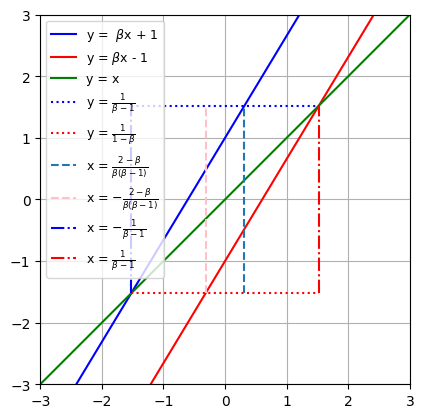
\includegraphics[scale=0.5]{Conclusion2.png}
            \caption{图像}
            \label{fig:C1onclusion2}
      \end{figure*}

      由图像可以看出,当$x\in(-\frac{1}{\beta-1},\frac{2-\beta}{\beta(\beta-1)})$,有$f_1(x)\in(-\frac{1}{\beta-1},\frac{1}{\beta-1})$,而当$x\in(-\frac{2-\beta}{\beta(\beta-1)},\frac{1}{\beta-1})$,有$f_{-1}(x)\in(-\frac{1}{\beta-1},\frac{1}{\beta-1})$。

      而我们又有$(-\frac{1}{\beta-1},\frac{2-\beta}{\beta(\beta-1)})\cup(-\frac{2-\beta}{\beta(\beta-1)},\frac{1}{\beta-1})=(-\frac{1}{\beta-1},\frac{1}{\beta-1})$,故可得,
      $$
            \forall x\in(-\frac{1}{\beta-1},\frac{1}{\beta-1}), \exists i\in\{-1,1\},\mbox{ 使得},f_i(x)\in(-\frac{1}{\beta-1},\frac{1}{\beta-1}).
      $$

      由此,因为$f_{\epsilon_k}(0)=1\in(-\frac{1}{\beta-1},\frac{1}{\beta-1})$,故有,存在一个序列$\{\epsilon_n\}_{n=0}^{k}\in\{-1,1\}$,使得,
      $$
            |\sum_{n=0}^k\epsilon_n\beta^n|<\frac{1}{\beta-1}.
      $$
\end{proof}

\begin{lemma}
      假设$T(x)=F(x)+G(x)$,若有$F:[0,1]\rightarrow\mathbb{R}$是Lipschtz连续的,其Lipschtz常数为$M>0$,$G:[0,1]\rightarrow\mathbb{R}$是连续函数,若$0<r<R<1$且$\frac{R}{r}\in\mathbb{Z}$,则我们有以下不等式:
      $$
                  \underset{a\in[0,1]\times\mathbb{R}}{\sup} N(S(a,\frac{R}{2})\cap\Gamma_T,r)
                  \ge\frac{1}{M+2} \underset{a\in[0.1]\times\mathbb{R}}{\sup}N(S(a,\frac{R}{2})\cap\Gamma_G,r)-\frac{M+2}{\lfloor M\rfloor+2}\frac{R}{r}.
      $$
\end{lemma}

其详细证明可查看[1,第六节]


假设$H_{a,b}(x)=\sum_{n=0}^\infty a^nh(b^nx)$,其中$h(x)$为可分割折线函数,
$\mathbb{I}=\{I_1,I_2,\cdots,I_N\}$为$h(x)$在$[0,1]$区间上按不可导点分割产生的区间族。

$I_J$为$h(x)$在$[0,1]$区间上的导数不为$0$的区间长度最大的区间,其上$h(x)$的导数为$K_M$,其关于$x=\frac{1}{2}$对称的区间为$I_{J'}$,其上$h(x)$的导数为$-K_M$。

$0<a<1,b>1,1<ab<2,n(\mathbb{I})|b$,则我们可得以下结论:
$$
      \mathrm{\dim_A\Gamma_{H_{a,b}(x)}}\ge1+\frac{1}{k}\Big(1-\log_b\frac{1}{2|I_J|}\Big).
$$




\begin{proof}

\end{proof}
